%\documentclass{acm_proc_article-sp}
\documentclass{sig-alternate}

\usepackage{url}
\usepackage[]{placeins}

\begin{document}
\title{Demo: Spectrum-Agile mm-Wave Packet Radio Implementation on USRPs}
%
% You need the command \numberofauthors to handle the 'placement
% and alignment' of the authors beneath the title.
%
% For aesthetic reasons, we recommend 'three authors at a time'
% i.e. three 'name/affiliation blocks' be placed beneath the title.
%
% NOTE: You are NOT restricted in how many 'rows' of
% "name/affiliations" may appear. We just ask that you restrict
% the number of 'columns' to three.
%
% Because of the available 'opening page real-estate'
% we ask you to refrain from putting more than six authors
% (two rows with three columns) beneath the article title.
% More than six makes the first-page appear very cluttered indeed.
%
% Use the \alignauthor commands to handle the names
% and affiliations for an 'aesthetic maximum' of six authors.
% Add names, affiliations, addresses for
% the seventh etc. author(s) as the argument for the
% \additionalauthors command.
% These 'additional authors' will be output/set for you
% without further effort on your part as the last section in
% the body of your article BEFORE References or any Appendices.

\numberofauthors{1} %  in this sample file, there are a *total*
% of EIGHT authors. SIX appear on the 'first-page' (for formatting
% reasons) and the remaining two appear in the \additionalauthors section.
%
\author{
% You can go ahead and credit any number of authors here,
% e.g. one 'row of three' or two rows (consisting of one row of three
% and a second row of one, two or three).
%
% The command \alignauthor (no curly braces needed) should
% precede each author name, affiliation/snail-mail address and
% e-mail address. Additionally, tag each line of
% affiliation/address with \affaddr, and tag the
% e-mail address with \email.
%
% 1st. author
\alignauthor
Julian Arnold, Ljiljana Simi\'{c}, Marina Petrova and Petri M\"ah\"onen\\
       \affaddr{Institute for Networked Systems, RWTH Aachen University}\\
       \affaddr{Kackertstrasse 9, 52072 Aachen, Germany}\\
       \email{\{jua, lsi, mpe, pma\}@inets.rwth-aachen.de}
}

\date{\today}

\maketitle
\begin{abstract}
We present a spectrum-agile mm-wave packet radio communication system and demonstrate it by using multimedia streaming. The developed platform is based on USRP software defined radios (SDRs) executing open-source GNU Radio code and cost-efficient commercial off-the-shelf components. Our system is able to operate in both the V- and E-bands, covering in practice the 60~GHz, 70~GHz and 80~GHz frequency bands. One of the main design goals has been to provide an SDR design that academic groups, particularly protocol designers, could use easily for future mm-wave system development and experimental verification.
\end{abstract}

% A category with the (minimum) three required fields
\category{C.2.1}{Network Architecture and Design}{Wireless communication}
\terms{Design, Experimentation}
\keywords{mm-wave, SDR, USRP, GNU Radio} % NOT required for Proceedings

\section{Introduction}
The demand for high speed connections and wireless capacity is rapidly growing, driven by the ever-increasing number of data-hungry applications. One promising solution to address this demand is to use mm-wave bands which provide a large amount of currently unoccupied bandwidth. However, while there is a growing body of literature on theoretical aspects of mm-wave communications (e.g. see~\cite{Rappaport14} and references therein) and several standards for short-range communication in the 60~GHz band are emerging~\cite{IEEE80211ad, IEEE802153c}, thus far very little \emph{practical} work has been published on mm-wave communication networks. Moreover, the published experimental work overwhelmingly focuses on mm-wave channel measurements and characterization~\cite{Rappaport01, Weiler14}; to the best of our knowledge, the only notable exceptions to this are the works in~\cite{Zhou12, Zhu14, Nitsche15, Zetterberg15}. We believe that this lack of publications focusing on practical aspects of mm-wave networks is largely due to the fact that researchers do not have access to open, configurable, and cost-efficient platforms that would enable experimental mm-wave research, not only at the PHY layer, but also across the upper protocol layers.

In~\cite{Zhou12, Zhu14} the authors reported on their measurements to demonstrate the feasibility of 60 GHz links for indoor data centre links and outdoor pico-cells, respectively. However, due to limited hardware availability, the work in~\cite{Zhou12, Zhu14} used closed point-to-point mm-wave transceivers~\cite{hxi, wilocity} that do not allow any modification of the lower layers. Moreover, these mm-wave devices are originally designed for point-to-point backhaul-like links~\cite{hxi}  and device-to-device communication~\cite{wilocity} and are not intended for general experimental work; beyond providing very basic characterization of achievable mm-wave link quality with their own specific design, the value of these platforms for more advanced mm-wave network research is thus extremely limited. In~\cite{Nitsche15} the authors demonstrated a technique that significantly reduces the time needed for 60~GHz link establishment by using 2.4/5~GHz Wi-Fi for direction estimation. However their mm-wave link was not packetized, but provided by connecting mm-wave converters~\cite{vubiqnetworks} to a signal generator and oscilloscope. Very recently the authors in~\cite{Zetterberg15} demonstrated an open-source 60~GHz transceiver design which is also compatible with USRP software defined radios (SDRs). Although this is indeed a big step forward, the authors mainly focused on the open hardware design and its evaluation and substantial effort would still be required to actually fabricate the proposed transceiver for use in research.

In this demo we present a spectrum-agile mm-wave packet radio system implemented on USRPs. Using our system, researchers can easily implement and practically evaluate novel mm-wave PHY and MAC layer protocols and study their performance in real-world environments. To the best of our knowledge, we are the first to demonstrate an open-source packetized, highly-configurable SDR system that can be readily made to operate in several mm-wave bands.

\section{Design and Implementation}
Figs.~\ref{fig:system}~and~\ref{fig:block} show the demonstration system and the corresponding functional block diagram, respectively.
\begin{figure}[!tb]
\center
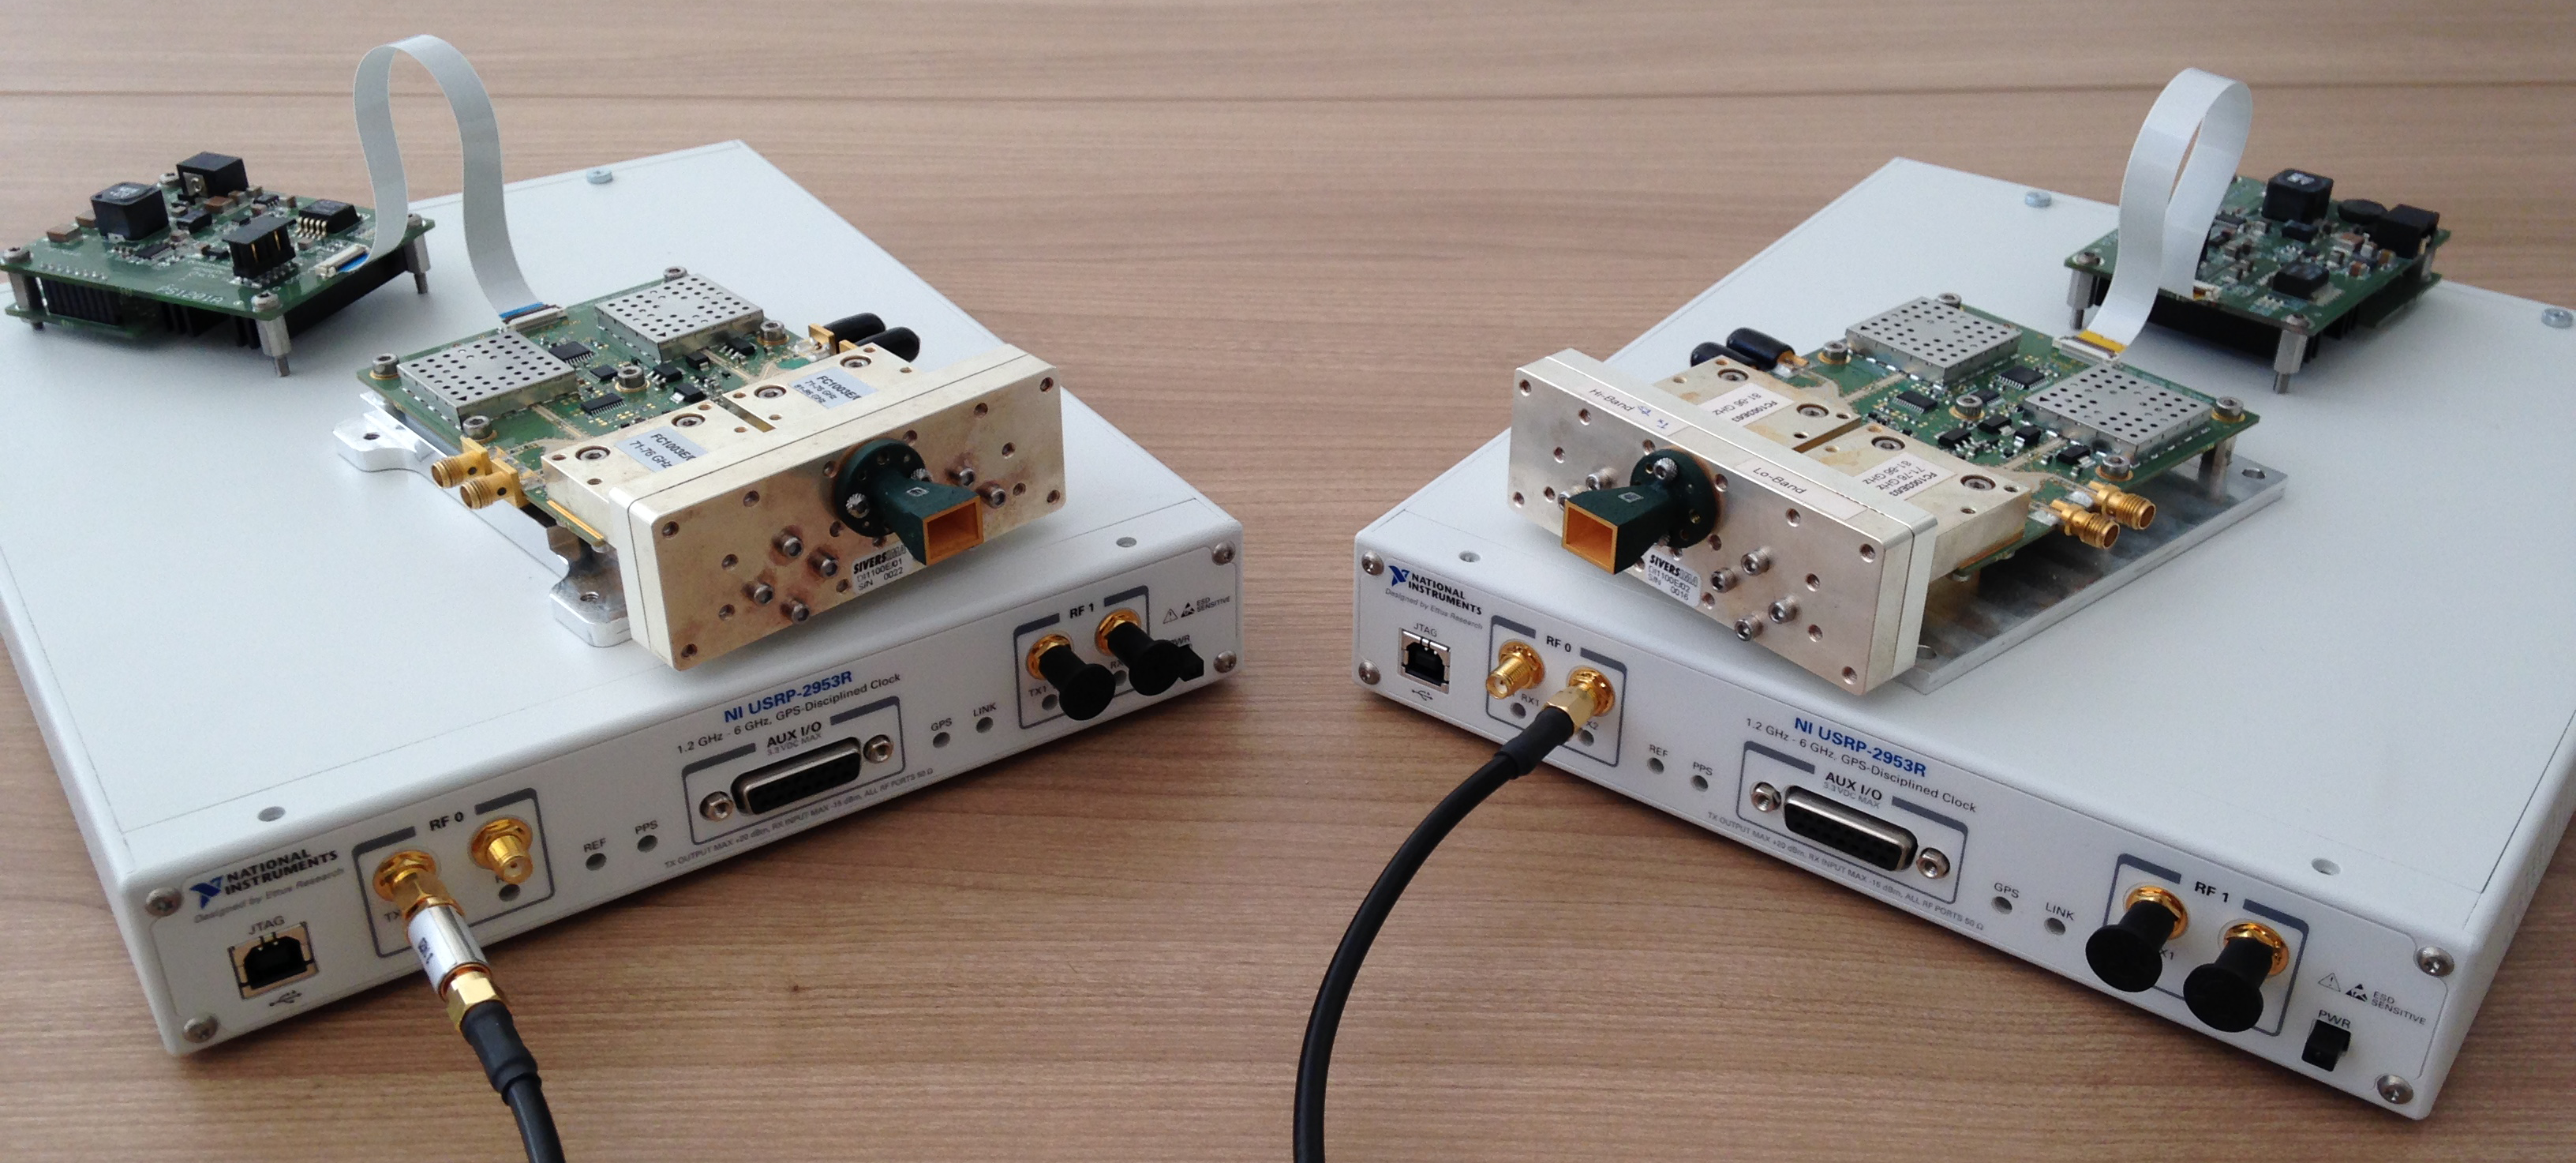
\includegraphics[width=0.4\textwidth]{system2.png}
\caption{Demonstrator equipment setup overview.}
\label{fig:system}
\end{figure}
\begin{figure}[!tb]
\center
\includegraphics[width=0.4\textwidth]{block-diagram}
\caption{Block diagram of the demonstrated mm-wave packet radio system.}
\label{fig:block}
\end{figure}
We use a host PC running GNU Radio~\cite{gnuradio} to generate a complex sample stream at baseband. The sample rate and thus the bandwidth of the stream is configurable in software. Our transceiver implementation follows a very modular concept based on the work demonstrated in \cite{Malsbury:phymac}, using recent GNU Radio features such as tagged streams and message passing. Fig.~\ref{fig:top-block} shows the GNU Radio flow graph of our overall transceiver implementation. In order to keep the individual flow graphs of manageable size and complexity, this top-level transceiver block is composed of the transmitter and receiver hierarchical blocks, shown in Figs.~\ref{fig:tx-path}~and~\ref{fig:rx-path}, respectively. These are in turn largely composed of stock GNU Radio blocks, although we have also implemented some custom blocks to ensure the transceiver functions properly with multimedia content.



As shown in the transmitter flow graph in Fig.~\ref{fig:tx-path}, the incoming packets from the upper layer are first segmented into smaller packets using the custom block \textit{packetizer python} before being converted into a tagged sample stream (the segmentation is necessary to ensure proper handling of the packets by the GNU Radio framework).%This requirement will become clear as we discuss the receiver section. T
Using a tagged stream MUX preamble, the header and padding bits are added to the sample stream. %We might as well merge all the packed building steps into our "packetizer python" block to reduce block count and to clean up the flow graph even more.
This final tagged stream is then modulated. Finally, the stream tags are adjusted using the \textit{Tagged Stream Multiply Length Tag} block.% before the tagged symbol stream is scaled and handed off to the SDR hardware. 

As shown in Fig.~\ref{fig:block}, this tagged symbol stream generated by the transmitter is then sent to an NI USRP-2953R \cite{ettus} SDR via Ethernet, with a maximum bandwidth of up to 40~MHz. However, one can easily replace the specific NI USRP used in the demonstration by a different NI USRP of the same product family containing other daughter cards, allowing a maximum bandwidth of 160~MHz. In the demonstration the USRP transfers the complex baseband signal to a passband signal at an intermediate frequency (IF) between 1.2~GHz and 6~GHz. The exact value of the IF can easily be adjusted via the GNU Radio program. Because of the wide IF range and the ability to change the frequency during run-time, our system can operate in a very spectrum-agile manner, allowing it to avoid interference with other transmissions.

An external upconverter \cite{siversima} is used to transfer the IF signal to the mm-wave RF band, which is then transmitted over the air using a waveguide-connected horn antenna. On the receiver side, the equivalent  processing is applied using a down-converter and the USRP as a receiver. The complex sample stream is fed back to a second host PC and processed in the receive path of our GNU Radio transceiver implementation.

As shown in the receiver flow graph in Figure~\ref{fig:rx-path}, the receiver hierarchical block applies matched filtering and frequency and time synchronization to the incoming symbol stream. The recently added \textit{Header/Payload Demux} (HPD) block is then used to split the incoming symbol stream into a payload and a header tagged stream, based on a trigger signal it receives from the upstream block \textit{Frame sync cc}. We implemented this custom block in order to detect a preamble added by the transmitter and to resolve phase ambiguity. We note that since the HPD block tries to copy a whole payload sequence at once into its output buffer, the payload size is limited by the maximum size of the shared memory available to a block in GNU Radio. It is this limited memory size that necessitates our implementation of packet fragmentation at the transmitter, as mentioned above. Therefore, the custom block \textit{unmake packet python} reassembles the packet fragments before handing off the reassembled packet to the upper layer on the receive side host PC, as shown in Fig.~\ref{fig:block}.

We note that the radio frontend we use directly supports the USRP-generated IF signal and gives us the freedom to change the central frequency in the mm-wave bands within the provided 1-6~GHz band (the actual maximum bandwidth of the signal depends on the baseband implementation).  Our system can thus be operated in the 60~GHz, 70~GHz, and 80~GHz bands simply by using the appropriate mm-wave converter boards without any further software changes to our SDR baseband implementation, which makes our system even more spectrum-agile.

We plan to release our baseband SDR implementation via \cite{gr-inets} as open-source code, with a detailed description of the overall hardware chain, as soon as a stable code version is approved. This will allow interested researchers to easily replicate the demonstrated experimental system, thereby enabling further practical research in mm-wave networks by modifying in software parameters like modulation scheme, channel bandwidth, synchronization method, as well as implementing novel MAC layer protocols.

\begin{figure*}[p]
\center
\includegraphics[scale=0.41]{tx_path.png}
\caption{GNU Radio flow graph of the transmitter hierarchical block.}
\label{fig:tx-path}
\end{figure*}

\begin{figure*}[p]
\center
\includegraphics[scale=0.41]{rx_path.png}
\caption{GNU Radio flow graph of the receiver hierarchical block.}
\label{fig:rx-path}
\end{figure*}

\begin{figure*}
\center
\includegraphics[scale=0.41]{transceiver.png}
\caption{Top-level GNU Radio flow graph of the overall transceiver implementation.}
\label{fig:top-block}
\end{figure*}

\section{Demonstration Description} 
During the demo session we will demonstrate the proposed system, showing its operation in several mm-wave bands by transmitting a multimedia stream over the air. % We will bring all the necessary equipment for our demonstration.
The audience will be able to closely inspect our hardware and software set-up and consider if a similar approach would be interesting for their own research. %Furthermore, we will show to the audience the real-time operation of our system by transmitting a multimedia-stream over the mm-wave link. 
As our design allows easy adjustment of PHY parameters via GNU Radio the audience will also be able to experiment with those %. Moreover, our GNU Radio implementation will allow the audience to 
and observe  in real-time the effect on several performance metrics of the mm-wave link.
%\balancecolumns


\section{Conclusions}
We have demonstrated an open-source mm-wave packet radio system, which will enable future practical research on mm-wave networks using readily available COTS components and open-source software. Furthermore, we have demonstrated the easy reconfigurability of our experimental system due to the use of SDRs, which will help drive novel MAC and PHY layer solutions for the mm-wave band.

%\begin{figure}
%\begin{tikzpicture}
%\draw[thick] (0, 0) rectangle (1,1) node[pos=.5] {USRP};
%\draw[thick, ->] (1,.5) -- (2,.5);
%\draw[thick] (2.4, 0.5) -- (3,.5);
%\end{tikzpicture}
%\caption{Do not forget!
%Make it explicit enough that readers
%can figure out what you are doing.}
%\end{figure}

\bibliographystyle{abbrv}
\bibliography{sigproc}
\balancecolumns
\end{document}